% Created by tikzDevice version 0.8.1 on 2015-05-24 13:11:58
% !TEX encoding = UTF-8 Unicode
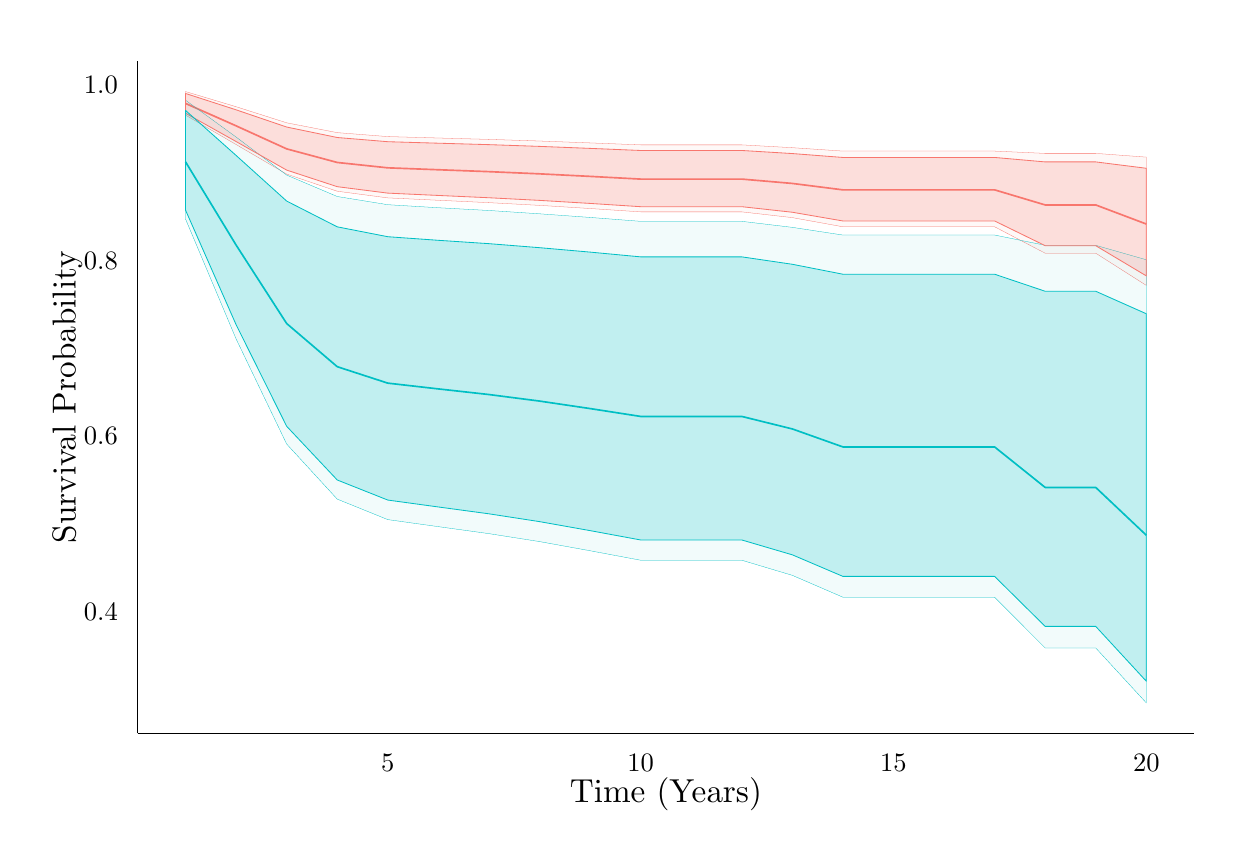
\begin{tikzpicture}[x=1pt,y=1pt]
\definecolor{fillColor}{RGB}{255,255,255}
\path[use as bounding box,fill=fillColor,fill opacity=0.00] (0,0) rectangle (433.62,289.08);
\begin{scope}
\path[clip] (  0.00,  0.00) rectangle (433.62,289.08);
\definecolor{drawColor}{RGB}{255,255,255}
\definecolor{fillColor}{RGB}{255,255,255}

\path[draw=drawColor,line width= 0.6pt,line join=round,line cap=round,fill=fillColor] (  0.00,  0.00) rectangle (433.62,289.08);
\end{scope}
\begin{scope}
\path[clip] ( 39.69, 34.03) rectangle (421.57,277.03);
\definecolor{fillColor}{RGB}{255,255,255}

\path[fill=fillColor] ( 39.69, 34.03) rectangle (421.58,277.03);
\definecolor{drawColor}{RGB}{248,118,109}

\path[draw=drawColor,line width= 0.6pt,line join=round] ( 57.05,261.70) --
	( 75.32,253.60) --
	( 93.59,245.28) --
	(111.86,240.37) --
	(130.13,238.43) --
	(148.41,237.74) --
	(166.68,237.05) --
	(184.95,236.26) --
	(203.22,235.34) --
	(221.49,234.36) --
	(239.77,234.36) --
	(258.04,234.36) --
	(276.31,232.79) --
	(294.58,230.47) --
	(312.86,230.47) --
	(331.13,230.47) --
	(349.40,230.47) --
	(367.67,225.02) --
	(385.94,225.02) --
	(404.22,218.12);
\definecolor{drawColor}{RGB}{0,191,196}

\path[draw=drawColor,line width= 0.6pt,line join=round] ( 57.05,240.59) --
	( 75.32,210.52) --
	( 93.59,182.17) --
	(111.86,166.57) --
	(130.13,160.63) --
	(148.41,158.54) --
	(166.68,156.51) --
	(184.95,154.15) --
	(203.22,151.44) --
	(221.49,148.60) --
	(239.77,148.60) --
	(258.04,148.60) --
	(276.31,144.08) --
	(294.58,137.58) --
	(312.86,137.58) --
	(331.13,137.58) --
	(349.40,137.58) --
	(367.67,122.94) --
	(385.94,122.94) --
	(404.22,105.67);
\definecolor{drawColor}{RGB}{248,118,109}
\definecolor{fillColor}{RGB}{248,118,109}

\path[draw=drawColor,line width= 0.1pt,line join=round,line cap=round,fill=fillColor,fill opacity=0.05] ( 57.05,265.99) --
	( 75.32,260.51) --
	( 93.59,254.70) --
	(111.86,251.15) --
	(130.13,249.72) --
	(148.41,249.21) --
	(166.68,248.71) --
	(184.95,248.12) --
	(203.22,247.44) --
	(221.49,246.73) --
	(239.77,246.73) --
	(258.04,246.73) --
	(276.31,245.71) --
	(294.58,244.48) --
	(312.86,244.48) --
	(331.13,244.48) --
	(349.40,244.48) --
	(367.67,243.65) --
	(385.94,243.65) --
	(404.22,242.30) --
	(404.22,195.94) --
	(385.94,207.58) --
	(367.67,207.58) --
	(349.40,217.13) --
	(331.13,217.13) --
	(312.86,217.13) --
	(294.58,217.13) --
	(276.31,220.44) --
	(258.04,222.52) --
	(239.77,222.52) --
	(221.49,222.52) --
	(203.22,223.73) --
	(184.95,224.87) --
	(166.68,225.85) --
	(148.41,226.71) --
	(130.13,227.57) --
	(111.86,229.98) --
	( 93.59,236.16) --
	( 75.32,246.85) --
	( 57.05,257.48) --
	cycle;
\definecolor{drawColor}{RGB}{0,191,196}
\definecolor{fillColor}{RGB}{0,191,196}

\path[draw=drawColor,line width= 0.1pt,line join=round,line cap=round,fill=fillColor,fill opacity=0.05] ( 57.05,262.86) --
	( 75.32,249.55) --
	( 93.59,235.81) --
	(111.86,228.07) --
	(130.13,225.11) --
	(148.41,224.01) --
	(166.68,223.02) --
	(184.95,221.82) --
	(203.22,220.51) --
	(221.49,219.10) --
	(239.77,219.10) --
	(258.04,219.10) --
	(276.31,216.92) --
	(294.58,214.14) --
	(312.86,214.14) --
	(331.13,214.14) --
	(349.40,214.14) --
	(367.67,210.44) --
	(385.94,210.44) --
	(404.22,205.22) --
	(404.22, 45.08) --
	(385.94, 64.94) --
	(367.67, 64.94) --
	(349.40, 83.28) --
	(331.13, 83.28) --
	(312.86, 83.28) --
	(294.58, 83.28) --
	(276.31, 91.18) --
	(258.04, 96.64) --
	(239.77, 96.64) --
	(221.49, 96.64) --
	(203.22,100.07) --
	(184.95,103.38) --
	(166.68,106.25) --
	(148.41,108.77) --
	(130.13,111.32) --
	(111.86,118.72) --
	( 93.59,138.62) --
	( 75.32,176.60) --
	( 57.05,219.91) --
	cycle;
\definecolor{drawColor}{RGB}{248,118,109}
\definecolor{fillColor}{RGB}{248,118,109}

\path[draw=drawColor,line width= 0.3pt,line join=round,line cap=round,fill=fillColor,fill opacity=0.20] ( 57.05,265.30) --
	( 75.32,259.39) --
	( 93.59,253.17) --
	(111.86,249.39) --
	(130.13,247.87) --
	(148.41,247.33) --
	(166.68,246.81) --
	(184.95,246.18) --
	(203.22,245.46) --
	(221.49,244.70) --
	(239.77,244.70) --
	(258.04,244.70) --
	(276.31,243.59) --
	(294.58,242.18) --
	(312.86,242.18) --
	(331.13,242.18) --
	(349.40,242.18) --
	(367.67,240.57) --
	(385.94,240.57) --
	(404.22,238.27) --
	(404.22,199.38) --
	(385.94,210.30) --
	(367.67,210.30) --
	(349.40,219.23) --
	(331.13,219.23) --
	(312.86,219.23) --
	(294.58,219.23) --
	(276.31,222.38) --
	(258.04,224.39) --
	(239.77,224.39) --
	(221.49,224.39) --
	(203.22,225.57) --
	(184.95,226.67) --
	(166.68,227.62) --
	(148.41,228.45) --
	(130.13,229.29) --
	(111.86,231.62) --
	( 93.59,237.61) --
	( 75.32,247.93) --
	( 57.05,258.15) --
	cycle;
\definecolor{drawColor}{RGB}{0,191,196}
\definecolor{fillColor}{RGB}{0,191,196}

\path[draw=drawColor,line width= 0.3pt,line join=round,line cap=round,fill=fillColor,fill opacity=0.20] ( 57.05,259.17) --
	( 75.32,242.90) --
	( 93.59,226.42) --
	(111.86,217.11) --
	(130.13,213.54) --
	(148.41,212.24) --
	(166.68,211.03) --
	(184.95,209.58) --
	(203.22,207.98) --
	(221.49,206.26) --
	(239.77,206.26) --
	(258.04,206.26) --
	(276.31,203.58) --
	(294.58,199.99) --
	(312.86,199.99) --
	(331.13,199.99) --
	(349.40,199.99) --
	(367.67,193.83) --
	(385.94,193.83) --
	(404.22,185.70) --
	(404.22, 52.91) --
	(385.94, 72.73) --
	(367.67, 72.73) --
	(349.40, 90.80) --
	(331.13, 90.80) --
	(312.86, 90.80) --
	(294.58, 90.80) --
	(276.31, 98.59) --
	(258.04,103.96) --
	(239.77,103.96) --
	(221.49,103.96) --
	(203.22,107.34) --
	(184.95,110.59) --
	(166.68,113.41) --
	(148.41,115.88) --
	(130.13,118.38) --
	(111.86,125.63) --
	( 93.59,145.03) --
	( 75.32,181.74) --
	( 57.05,223.13) --
	cycle;
\end{scope}
\begin{scope}
\path[clip] (  0.00,  0.00) rectangle (433.62,289.08);
\definecolor{drawColor}{RGB}{0,0,0}

\path[draw=drawColor,line width= 0.6pt,line join=round] ( 39.69, 34.03) --
	( 39.69,277.03);
\end{scope}
\begin{scope}
\path[clip] (  0.00,  0.00) rectangle (433.62,289.08);
\definecolor{drawColor}{RGB}{0,0,0}

\node[text=drawColor,anchor=base east,inner sep=0pt, outer sep=0pt, scale=  0.96] at ( 32.57, 74.72) {0.4};

\node[text=drawColor,anchor=base east,inner sep=0pt, outer sep=0pt, scale=  0.96] at ( 32.57,138.29) {0.6};

\node[text=drawColor,anchor=base east,inner sep=0pt, outer sep=0pt, scale=  0.96] at ( 32.57,201.85) {0.8};

\node[text=drawColor,anchor=base east,inner sep=0pt, outer sep=0pt, scale=  0.96] at ( 32.57,265.42) {1.0};
\end{scope}
\begin{scope}
\path[clip] (  0.00,  0.00) rectangle (433.62,289.08);
\definecolor{drawColor}{RGB}{0,0,0}

\path[draw=drawColor,line width= 0.6pt,line join=round] ( 39.69, 34.03) --
	(421.57, 34.03);
\end{scope}
\begin{scope}
\path[clip] (  0.00,  0.00) rectangle (433.62,289.08);
\definecolor{drawColor}{RGB}{0,0,0}

\node[text=drawColor,anchor=base,inner sep=0pt, outer sep=0pt, scale=  0.96] at (130.13, 20.31) {5};

\node[text=drawColor,anchor=base,inner sep=0pt, outer sep=0pt, scale=  0.96] at (221.49, 20.31) {10};

\node[text=drawColor,anchor=base,inner sep=0pt, outer sep=0pt, scale=  0.96] at (312.86, 20.31) {15};

\node[text=drawColor,anchor=base,inner sep=0pt, outer sep=0pt, scale=  0.96] at (404.22, 20.31) {20};
\end{scope}
\begin{scope}
\path[clip] (  0.00,  0.00) rectangle (433.62,289.08);
\definecolor{drawColor}{RGB}{0,0,0}

\node[text=drawColor,anchor=base,inner sep=0pt, outer sep=0pt, scale=  1.20] at (230.63,  9.03) {Time (Years)};
\end{scope}
\begin{scope}
\path[clip] (  0.00,  0.00) rectangle (433.62,289.08);
\definecolor{drawColor}{RGB}{0,0,0}

\node[text=drawColor,rotate= 90.00,anchor=base,inner sep=0pt, outer sep=0pt, scale=  1.20] at ( 17.30,155.53) {Survival Probability};
\end{scope}
\end{tikzpicture}
